% !TEX encoding = UTF-8 Unicode
\documentclass[a4paper,12pt]{extreport}
\usepackage[utf8]{inputenc}
\usepackage{color}
\usepackage[T2A]{fontenc}
\usepackage[intlimits]{amsmath}
\usepackage{amssymb}
\usepackage{dsfont}
\usepackage{bm}
\usepackage{indentfirst}
% \usepackage[1cm]{fullpage}
\usepackage{geometry}
\usepackage{soul}
\usepackage[normalem]{ulem}
\usepackage[english,russian]{babel}
\usepackage{hyperref}
\hypersetup{
    colorlinks=true,
    linkcolor=blue,
    filecolor=magenta,      
    urlcolor=cyan,
}
\usepackage{mathtools}
\usepackage{graphicx}
\usepackage{multicol}
\usepackage{float}
\graphicspath{{Pictures/}}

\linespread{1.15}                    % Полуторный интвервал (ГОСТ Р 7.0.11-2011, 5.3.6)
% \Large


% \renewcommand{\labelenumi}{(\alph{enumi})} % Use letters for enumerate
% \DeclareMathOperator{\Sample}{Sample}
\let\vaccent=\v % rename builtin command \v{} to \vaccent{}
\usepackage{enumerate}
\renewcommand{\v}[1]{\ensuremath{\mathbf{#1}}} % for vectors
\newcommand{\gv}[1]{\ensuremath{\mbox{\boldmath$ #1 $}}} 
% for vectors of Greek letters
\newcommand{\uv}[1]{\ensuremath{\mathbf{\hat{#1}}}} % for unit vector
\newcommand{\abs}[1]{\left| #1 \right|} % for absolute value
\newcommand{\avg}[1]{\left< #1 \right>} % for average
\let\underdot=\d % rename builtin command \d{} to \underdot{}
\renewcommand{\d}[2]{\frac{d #1}{d #2}} % for derivatives
\newcommand{\dd}[2]{\frac{d^2 #1}{d #2^2}} % for double derivatives
\newcommand{\pd}[2]{\frac{\partial #1}{\partial #2}} 
% for partial derivatives
\newcommand{\pdd}[2]{\frac{\partial^2 #1}{\partial #2^2}} 
% for double partial derivatives
\newcommand{\pdc}[3]{\left( \frac{\partial #1}{\partial #2}
 \right)_{#3}} % for thermodynamic partial derivatives
\newcommand{\ket}[1]{\left| #1 \right>} % for Dirac bras
\newcommand{\bra}[1]{\left< #1 \right|} % for Dirac kets
\newcommand{\braket}[2]{\left< #1 \vphantom{#2} \right|
 \left. #2 \vphantom{#1} \right>} % for Dirac brackets
\newcommand{\matrixel}[3]{\left< #1 \vphantom{#2#3} \right|
 #2 \left| #3 \vphantom{#1#2} \right>} % for Dirac matrix elements
\newcommand{\grad}[1]{\gv{\nabla} #1} % for gradient
\let\divsymb=\div % rename builtin command \div to \divsymb
\renewcommand{\div}[1]{\gv{\nabla} \cdot \v{#1}} % for divergence
\newcommand{\curl}[1]{\gv{\nabla} \times \v{#1}} % for curl
\let\baraccent=\= % rename builtin command \= to \baraccent
\renewcommand{\=}[1]{\stackrel{#1}{=}} % for putting numbers above =
\providecommand{\wave}[1]{\v{\tilde{#1}}}
\providecommand{\fr}{\frac}
\providecommand{\RR}{\mathbb{R}}
\providecommand{\NN}{\mathbb{N}}
\providecommand{\seq}{\subseteq}
\providecommand{\e}{\varepsilon}

% LaTeX internal stuff
\newcommand{\innermid}{\nonscript\;\delimsize\vert\nonscript\;}
\newcommand{\activatebar}{%
  \begingroup\lccode`\~=`\|
  \lowercase{\endgroup\let~}\innermid 
  \mathcode`|=\string"8000
}

% Probability theory
\newcommand{\Expect}{\mathop{{}\mathrm{E}}}
\newcommand{\Expectmore}{\operatorname{E}\expectarg}
\newcommand{\covmore}{\operatorname{cov}\expectarg}
\DeclarePairedDelimiterX{\expectarg}[1]{[}{]}{%
  \ifnum\currentgrouptype=16 \else\begingroup\fi
  \activatebar#1
  \ifnum\currentgrouptype=16 \else\endgroup\fi
}
\newcommand{\Proba}{\mathrm{P}}
\newcommand{\Var}{\mathop{{}\mathrm{V}}}

% Stochastic processes
\newcommand{\generaltime}{t \geqslant 0}
\newcommand{\discretetime}{t = 1,\,2,\,\ldots}
\newcommand{\conttime}{t \in \realline^{+}}
\newcommand{\finiteconttime}[1]{0 \leqslant t \leqslant #1}
\newcommand{\finitediscretetime}[1]{\running{t}{1}{#1}}

\newcommand{\newprocess}[1]{
    \ensuremath{
        #1 = \left(#1 _t\right)_{\generaltime}
    }
}
\newcommand{\newprocessd}[1]{
    \ensuremath{
        #1 = \left(#1 _t\right)_{\discretetime}
    }
}
\newcommand{\newprocessfc}[2]{
    \ensuremath{
        #1 = \left(#1 _t\right)_{\finiteconttime{#2}}
    }
}

\newcommand{\trajectory}[1]{\big\{#1_s,\,0\leqslant s \leqslant t\big\}}
\newcommand{\firsttime}[1]{\ensuremath{\inf \{\generaltime: #1\}}}

\newcommand{\filtration}[1]{\mathcal{#1}}
\newcommand{\filtrationprocess}[2]{\filtration{#1}^{#2}}
\newcommand{\filtrationflow}[1]{\newprocess{\filtration{F}}}

\newcommand{\fbm}{B^H}

\geometry{paper=a4paper,top=1cm,bottom=2cm,left=2cm,right=2cm}

\begin{document}


\begin{center}
    \begin{tabular}{|p{15.5cm}|}
        \hline
        \textbf{ФКН ВШЭ, 3 курс, 3 модуль}\\
        \begin{center} \Large Материалы к экзамену
        \end{center}\\
        \textbf{Вероятностные модели и статистика случайных процессов, весна 2017}\\
        \hline
    \end{tabular}
\end{center}

% Время выдачи задания: 10 февраля (пятница), 12:10.

% Срок сдачи: \textcolor{blue}{\bf 10 февраля (пятница), 12:40.}

% \section*{Правила сдачи}

% \begin{enumerate}
% \item Работу необходимо сдать преподавателю на листе бумаги
% до дедлайна.
% \item Сверху листа укажите ваши фамилию и имя.
% \item \textbf{Каждая из задач имеет стоимость 1 балл.}
% Максимально допустимая оценка за работу -- 10 баллов. 
% \end{enumerate}


\section*{\centeringТеоретический минимум}


\begin{enumerate}
    % \item Сформулируйте определение случайного процесса как случайной функции.
    % \item Сформулируйте определение сечения случайного процесса.
    % \item Сформулируйте определение траектории случайного процесса.

    % \item Сформулируйте определение случайного процесса с непрерывным временем.
    % \item Сформулируйте определение случайного процесса с дискретным временем.
    % \item Сформулируйте определение случайного поля.
    % \item Сформулируйте определение векторнозначного случайного процесса.

    % \item Приведите пример случайного процесса с непрерывным временем.
    % \item Приведите пример случайного процесса с дискретным временем.
    % \item Приведите пример случайного поля.
    % \item Приведите пример векторнозначного случайного процесса.

    % \item Сформулируйте определение семейства конечномерных распределений случайного процесса.
    % \item Приведите пример функции, задающей конечномерные распределения случайного процесса.

    % \item Сформулируйте определение математического ожидания случайного процесса.
    % \item Сформулируйте определение дисперсии случайного процесса.
    % \item Сформулируйте определение ковариационной функции случайного процесса.
    
    % \item Сформулируйте определение непрерывного в среднем квадратичном случайного процесса.
    % \item Сформулируйте определение случайного процесса с непрерывными траекториями.
    % \item Сформулируйте определение стохастически непрерывного случайного процесса.

    % \item Приведите пример непрерывного в среднем квадратичном случайного процесса.
    % \item Приведите пример случайного процесса с непрерывными траекториями.
    % \item Приведите пример стохастически непрерывного случайного процесса.

    % \item Сформулируйте определение гауссовской случайной величины.
    % \item Сформулируйте определение гауссовского случайного вектора.
    % \item Запишите выражение для характеристической функции гауссовской
    % случайной величины.
    % % \item Сформулируйте необходимые и достаточные условия гауссовости случайного вектора.

    % % \item Сформулируйте основное утверждение теоремы о нормальной корреляции
    % % в случае пары гауссовских случайных величин.
    % % \item Сформулируйте основное утверждение теоремы о нормальной корреляции
    % % в случае пары гауссовских случайных векторов.

    % \item Сформулируйте определение винеровского процесса.
    % \item Сформулируйте определение гауссовского процесса.
    % \item Приведите пример гауссовского процесса.
    % \item Сформулируйте определение процесса Орнштейна-Уленбека.

    % \item Сформулируйте определение последовательности независимых 
    % одинаково распределенных случайных величин.
    % \item Сформулируйте определение сильно стационарного случайного процесса.
    % \item Сформулируйте определение ковариационно стационарного случайного процесса.
    % \item Приведите пример сильно стационарного случайного процесса.
    % \item Приведите пример ковариационно стационарного случайного процесса.
    % \item Перечислите свойства ковариационной функции 
    % слабо стационарного случайного процесса.
    % \item Сформулируйте определение случайного процесса,
    % эргодичного в среднем квадратичном по математическому ожиданию.
    % \item Приведите пример процесса, являющегося эргодичным по математическому ожиданию
    % в среднем квадратичном.
    % % \item Сформулируйте необходимые и достаточные условия эргодичности
    % % случайного процесса в среднем по математическому ожиданию.
    % % \item Сформулируйте необходимые и достаточные условия эргодичности
    % % слабо стационарного случайного процесса в среднем по математическому ожиданию.

    % \item Сформулируйте определение процесса восстановления.
    % \item Сформулируйте определение пуассоновского процесса.
    % \item Запишите выражение для математического ожидания
    % однородного пуассоновского процесса с интенсивностью $\lambda > 0$.
    % \item Запишите выражение для распределения сечения
    % однородного пуассоновского процесса с интенсивностью $\lambda > 0$
    % в момент $t$.
    % \item Сформулируйте основные свойства приращений пуассоновского процесса.

    % \item Сформулируйте определение приращений случайного процесса.
    % \item Сформулируйте определение процесса с независимыми приращениями.
    % \item Сформулируйте определение процесса со стационарными приращениями.

    % \item Сформулируйте определение дискретной марковской цепи.
    % \item Сформулируйте определение марковского свойства.
    % % \item Сформулируйте теорему о вероятности последовательности
    % % состояний дискретной марковской цепи.
    % % \item Сформулируйте теорему о вероятности перехода однородной дискретной марковской цепи
    % % в заданное состояние за $n$ шагов.

    % \item Сформулируйте определения существенного и несущественного состояний марковской цепи.
    % \item Сформулируйте определения возвратного и невозвратного состояний марковской цепи.
    % \item Сформулируйте определение сообщающихся состояний марковской цепи.
    % \item Сформулируйте определение неприводимой дискретной марковской цепи.
    % \item Сформулируйте определения периодического и непериодического состояний марковской цепи.
    % % \item Сформулируйте утверждение о разбиении множества 
    % % состояний дискретной марковской цепи на классы сообщающихся состояний. Какое отношение
    % % существует между состояниями внутри каждого из таких классов?
    % \item Приведите пример дискретной марковской цепи.
    % \item Приведите пример дискретной марковской цепи с периодическими состояниями.
    % \item Приведите пример дискретной марковской цепи с невозвратными состояниями.

    % \item Сформулируйте определение дискретного случайного блуждания с дискретным временем.
    % % \item Сформулируйте условия возвратности некоторого состояния дискретной марковской цепи,
    % % используя матрицу перехода за один шаг.
    % % \item Сформулируйте условия возвратности некоторого состояния дискретной марковской цепи,
    % % используя вероятности вернуться в это состояние за конечное число шагов.
    % % \item Сформулируйте условия возвратности некоторого состояния дискретной марковской цепи,
    % % используя вероятности вернуться в это состояние за конечное число шагов.

    % \item Сформулируйте определение эргодической марковской цепи.
    % \item Сформулируйте определение стационарного распределения вероятностей
    % дискретной марковской цепи.
    % % \item Сформулируйте первую эргодическую теорему для дискретной марковской цепи.

    % \item Запишите выражение для авторегрессионной модели AR($p$).
    % \item Запишите выражение для модели скользящего среднего MA($q$).
    % \item Запишите выражение для смешанной модели авторегрессии и скользящего среднего ARMA($p, q$).
    % \item Запишите выражение для смешанной модели интегральной авторегрессии
    % и скользящего среднего ARIMA($p, d, q$).
    % \item Запишите выражение для авторегрессионной модели условной неоднородности ARCH($p$).
    % \item Запишите выражение для обобщенной авторегрессионной модели
    % условной неоднородности GARCH($p, q$).

    % \item Сформулируйте определение скрытой марковской модели.

    % \item Запишите выражение для линейной неоднородной модели динамической системы
    % в фильтре Калмана.
    % \item Запишите условия, при которых процесс, моделирующий состояние
    % в модели динамической системы, является марковским.


    %%%%%%%%%%%%%%%%%%%%%%%%%%%%%%%%
    % Тема 8: проверка гипотез
    %%%%%%%%%%%%%%%%%%%%%%%%%%%%%%%%
    \item Сформулируйте определение решающего правила
    в~задаче различения двух гипотез.

    \item Сформулируйте определения вероятностей ошибок
    первого и~второго родов в~задаче различения двух гипотез~$\mathbb{H}_0$
    и~$\mathbb{H}_{\infty}$.

    \item Сформулируйте определение решающего правила в~задаче
    различения двух гипотез, минимизирующего сумму ошибок
    1~и~2~родов.

    \item Сформулируйте определение решающего правила
    в~задаче различения двух гипотез, оптимального
    в~условно-экстремальной постановке.

    \item Сформулируйте определение рандомизированного 
    решающего правила в~задаче различения двух гипотез.
    
    \item Сформулируйте определение рандомизированного решающего правила
    в~задаче различения двух гипотез, оптимального
    в~условно-экстремальной постановке.

    \item Сформулируйте фундаментальную лемму Неймана-Пирсона.

\end{enumerate}

\newpage

\section*{\centeringТеоретический максимум}

\begin{enumerate}
    % \item С использованием теоремы А.~Н.~Колмогорова 
    % продемонстрировать невозможность существования непрерывного случайного процесса
    % с сечениями, являющимися последовательностью независимых случайных величин.

    % \item Сформулировать и доказать необходимые и достаточные условия непрерывности
    % случайного процесса в среднем квадратичном.

    % \item С использованием определения стохастически непрерывного процесса
    % доказать, что свойства стохастической непрерывности и независимости 
    % сечений случайного процесса (при близких значениях времени) являются несовместными.

    % \item Сформулировать и доказать утверждение о необходимых
    % и достаточных условиях гауссовости случайного вектора.

    % \item Сформулировать и доказать теорему о нормальной корреляции
    % в случае пары гауссовских случайных величин.

    % \item Сформулировать и доказать теорему о нормальной корреляции
    % в случае пары гауссовских случайных векторов.

    % \item Сформулировать определения и свойства винеровского
    % и гауссовского процессов. Привести примеры гауссовских процессов.
    % Описать полный набор параметров, однозначно определяющих гауссовский 
    % процесс, обосновать это описание.

    % \item Получить явный аналитический вид системы конечномерных
    % распределений процесса Орнштейна-Уленбека.

    \item Перечислить классы стационарности случайных процессов,
    описать связь между ними.
    Привести примеры процессов, относящихся к каждому классу,
    но не относящихся к остальным.

    \item Сформулировать и доказать свойства
    (распределение, матожидание и дисперсию) пуассоновского
    потока событий с интенсивностью $\lambda > 0$ в момент $t$.

    % \item Получить явный аналитический вид системы конечномерных
    % распределений пуассоновского процесса.

    % \item Сформулировать и доказать теорему о вероятности 
    % наблюдения заданной последовательности
    % состояний дискретной марковской цепи.

    \item Сформулировать и доказать теорему о вероятности перехода 
    дискретной марковской цепи из одного состояния в другое за $n$ шагов.

    % \item Описать классификацию состояний дискретной марковской цепи.

    \item Сформулировать и доказать условия возвратности либо
    невозвратности случайного блуждания.

    % \item Сформулировать и доказать утверждение
    % о том, что возвратность или невозвратность состояния дискретной марковской цепи 
    % следует из равенства или неравенства бесконечности
    % величины $\sum\limits_{i=1}^n p^{(n)}_{ii}$, соответственно.

    % \item Сформулировать и доказать утверждение
    % о том, что возвратность или невозвратность состояния дискретной марковской цепи 
    % равносильна тому, что вероятность $f_i$ события $\{\exists n \in \mathbb{N}: X_n = i\}$,
    % где $n$ -- некоторый момент времени, $i$ -- рассматриваемое состояние,
    % равняется либо меньше единицы, соответственно.

    \item Сформулировать и доказать утверждение
    о том, что (1) если одно из состояний цепи нулевое, то и все остальные нулевые,
    (2) если одно из состояний возвратное, то и все остальные возвратные,
    (3) если одно из состояний периодическое с периодом $d$, то и все остальные
    периодические с периодом $d$.

    % \item Вывести формулу средней длительности пребывания дискретной марковской цепи
    % в заданном состоянии.

    \item Описать вычислительную разностную схему, позволяющую
    сгенерировать реализацию гауссовского случайного процесса 
    с помощью стохастического интегрирования по броуновскому движению
    (на примере процесса Орнштейна-Уленбека).

    % \item Описать вычислительную схему, позволяющую
    % сгенерировать реализацию гауссовского случайного процесса 
    % с помощью разложения Холецкого
    % (на примере процесса фрактального броуновского движения).

    \item Описать вычислительную схему, позволяющую
    сгенерировать реализацию однородного пуассоновского случайного процесса.

    % \item Описать вычислительную схему, позволяющую
    % сгенерировать реализацию неоднородного пуассоновского случайного процесса.

    % \item Пусть $(h_1, \ldots, h_n)$ -- реализация, полученная 
    % в результате наблюдений величин $h_k$ из модели MA($q$)
    % в моменты $k=1, \ldots, n$, и $\overline{h_n} = \frac 1 n \sum\limits_{k=1} ^n h_k$ --
    % временное среднее. 
    % Доказать, что стремление величины $\Delta_n^2 = \Expect |\overline{h_n} - \mu|^2$ к нулю 
    % при $n \to \infty$ равносильно стремлению к нулю суммы $\frac 1 n \sum\limits_{k=1} ^n R(k)$,
    % где $R(k) = \mathrm{cov}(h_{n + k}, h_n)$. Здесь $\Expect h_n = \mu$.

    % \item Модель системы массового обслуживания, рассмотренная на лекции.

    % \item Вывести уравнения Юла-Уолкера для авторегрессионной модели AR($p$).

    \item Пусть $(\bm{S}_n, \bm{X}_n)$~--
    скрытая марковская модель с $M$ состояниями и матрицей
    перехода за один шаг $P = (p_{ij}), i, j = 1, \ldots, M$,
    в которой условное распределение $p(X_i | S_i = s_i)$ является
    нормальным $\mathcal{N}(\mu_{s_i}, \sigma^2)$.
    Описать алгоритм сегментации временного ряда, в котором 
    параметры $\bm{\theta} = (P, \bm{\mu}, \sigma)$ известны,
    и требуется по выборке $(x_1, \ldots, x_n)$ 
    оценить значения $(s_1, \ldots, s_n)$ скрытых состояний
    $(S_1, \ldots, S_n)$  марковской цепи. Описать необходимые
    для решения заданной задачи предположения.

    % \item Пусть $(\bm{S}_n, \bm{X}_n)$~--
    % скрытая марковская модель с $M$ состояниями и матрицей
    % перехода за один шаг $P = (p_{ij}), i, j = 1, \ldots, M$,
    % в которой условное распределение $p(X_i | S_i = s_i)$ является
    % нормальным $\mathcal{N}(\mu_{s_i}, \sigma^2)$.
    % Описать алгоритм сегментации временного ряда, в котором 
    % параметры $\bm{\theta} = (P, \bm{\mu}, \sigma)$ неизвестны,
    % и требуется по выборке $(x_1, \ldots, x_n)$ 
    % оценить значения этих параметров
    % и значения $(s_1, \ldots, s_n)$ скрытых состояний
    % $(S_1, \ldots, S_n)$ марковской цепи. Описать необходимые
    % для решения заданной задачи предположения.

\end{enumerate}

\newpage

\section*{\centeringЗадачи}

\begin{enumerate}
    % \item Подсчитайте математическое ожидание, дисперсию
    % и ковариационную функцию случайного процесса
    % $\newprocess{Y}$, задаваемого соотношением
    % \[
    % Y_t = a(t) X_t + b(t),
    % \]
    % где $\newprocess{X}$ -- случайный процесс с математическим ожиданием 
    % $m(t) = \Expect X_t$, дисперсией $\sigma^2(t) = \Expectmore{X_t - \Expect X_t}^2$
    % и ковариационной функцией $R(t_1, t_2) = 
    % \Expectmore{(X_{t_1} - \Expect X_{t_1})(X_{t_2} - \Expect X_{t_2})}$.

    % \item Доказать, что пуассоновский поток событий является стохастически 
    % непрерывным случайным процессом.

    % \item Пусть $\bm{\xi} = (\xi_1, \xi_2)^{\intercal}$ -- гауссовский случайный вектор
    % с математическим ожиданием $\Expect \bm{\xi} = \bm{\mu} = (\mu_1, \mu_2)^{\intercal}$
    % и ковариационной матрицей 
    % \[
    % \Expectmore{(\bm{\xi} - \bm{\mu})(\bm{\xi} - \bm{\mu})^{\intercal}} = 
    %   \begin{bmatrix}
    %     \sigma_1^2 & \rho \sigma_1 \sigma_2\\
    %     \rho \sigma_1 \sigma_2 & \sigma_2^2
    %   \end{bmatrix}.
    % \]
    % Выписать явное аналитическое выражение для двумерной плотности
    % распределения случайного вектора $\bm{\xi}$.

    \item Пусть $\bm{\xi} = (\xi_1, \xi_2)^{\intercal}$ -- гауссовский случайный вектор
    с математическим ожиданием $\Expect \bm{\xi} = \bm{\mu} = (\mu_1, \mu_2)^{\intercal}$
    и ковариационной матрицей 
    \[
    \Expectmore{(\bm{\xi} - \bm{\mu})(\bm{\xi} - \bm{\mu})^{\intercal}} = 
      \begin{bmatrix}
        \sigma_1^2 & \rho \sigma_1 \sigma_2\\
        \rho \sigma_1 \sigma_2 & \sigma_2^2
      \end{bmatrix}.
    \]
    Подсчитать явное аналитическое выражение для условной плотности
    $f_{\xi_2|\xi_1}(x_2 | x_1)$
    распределения случайного вектора $\xi_2$ при условии $\xi_1 = x_1$.

    % \item Пусть $N^1, N^2, \ldots, N^n$ -- независимые пуассоновские потоки событий
    % с интенсивностями $\lambda_1, \lambda_2, \ldots, \lambda_n$, соответственно.
    % Определить тип и параметры процесса $N_t = \sum\limits_{i=1}^n N^i_t$.


    \item Подсчитать корреляции процесса MA(2). 
    \item Подсчитать корреляции процесса MA($q$). 

    % \item Подсчитать математическое ожидание процесса AR(1) и его предел при $n \to \infty$,
    % где $n$ -- время. 
    % \item Подсчитать дисперсию процесса AR(1) и ее предел при $n \to \infty$,
    % где $n$ -- время. 
    % \item Подсчитать ковариацию процесса AR(1) и ее предел при $n \to \infty$,
    % где $n$ -- время.

    % \item Записать правдоподобие $L(h_1, \ldots, h_n | \bm{\theta})$
    % выборки $(h_1, \ldots, h_n)$ из
    % авторегрессионной модели AR($p$), где $\bm{\theta} = (a_0, \ldots, a_p, \sigma)$.

    % \item Подсчитать математическое ожидание процесса ARMA(1,1) и его предел при $n \to \infty$,
    % где $n$ -- время. 
    % \item Подсчитать дисперсию процесса ARMA(1,1) и е предел при $n \to \infty$,
    % где $n$ -- время. 
    \item Подсчитать ковариацию процесса ARMA(1,1) и ее предел при $n \to \infty$,
    где $n$ -- время.

    % \item Подсчитать математическое ожидание квадрата процесса ARCH(1)
    % (величину $\Expect h^2_n$)
    % и его предел при $n \to \infty$, где $n$ -- время. 
    % \item Подсчитать математическое ожидание 4 степени процесса ARCH(1)
    % (величину $\Expect h^4_n$)
    % и его предел при $n \to \infty$, где $n$ -- время. 
    % \item Подсчитать дисперсию квадрата процесса ARCH(1)
    % (величину $\mathrm{D} h^2_n$)
    % и ее предел при $n \to \infty$, где $n$ -- время. 
    % \item Подсчитать первую корреляцию процесса ARCH(1)
    % (величину $\rho_1 = \Expect h^2_n h^2_{n - 1}$)
    % и ее предел при $n \to \infty$, где $n$ -- время. 
    % \item Записать правдоподобие $L(h_1, \ldots, h_n | \bm{\theta})$
    % выборки $(h_1, \ldots, h_n)$ из
    % модели ARCH(1), где $\bm{\theta} = (\alpha_0, \alpha_1)$.

    % \item Подсчитать математическое ожидание квадрата процесса GARCH(1,1)
    % (величину $\Expect h^2_n$)
    % и его предел при $n \to \infty$, где $n$ -- время. 
    % \item Подсчитать математическое ожидание 4 степени процесса GARCH(1,1)
    % (величину $\Expect h^4_n$)
    % и его предел при $n \to \infty$, где $n$ -- время. 
    % \item Подсчитать первую корреляцию процесса GARCH(1,1)
    % (величину $\rho_1 = \Expect h^2_n h^2_{n - 1}$)
    % и ее предел при $n \to \infty$, где $n$ -- время. 
    % \item Записать правдоподобие $L(h_1, \ldots, h_n | \bm{\theta})$
    % выборки $(h_1, \ldots, h_n)$ из
    % модели GARCH(1,1), где $\bm{\theta} = (\alpha_0, \alpha_1, \beta_1)$.

    % \item Записать правдоподобие $L(\bm{S}_n, \bm{X}_n| \bm{\theta})$
    % выборки $(\bm{S}_n, \bm{X}_n) = (s_1, \ldots, s_n, x_1, \ldots, x_n)$ из
    % скрытой марковской модели с $M$ состояниями и матрицей
    % перехода за один шаг $P = (p_{ij}), i, j = 1, \ldots, M$,
    % где $\bm{\theta} = (P, \bm{\mu}, \sigma)$
    % а условное распределение $p(X_i | S_i = s_i)$ является
    % нормальным $\mathcal{N}(\mu_{s_i}, \sigma^2)$.

    \item Получить формулы для математического ожидания и ковариационной матрицы
    вектора состояния динамической системы в фильтре Калмана.
    % \item Получить формулы для условного относительно наблюдений $z_1, \ldots, z_{k-1}$
    % математического ожидания и ковариационной матрицы
    % вектора состояния динамической системы в фильтре Калмана.
    % \item Получить формулы для условного относительно наблюдений $z_1, \ldots, z_k$
    % математического ожидания и ковариационной матрицы
    % вектора состояния динамической системы в фильтре Калмана.

    \item Приведите пример некоррелированных, но зависимых случайных величин.

    % \item Приведите пример процесса, являющегося сильно стационарным, 
    % но не эргодичным по математическому ожиданию в среднем квадратичном.

    % \item \label{mc_task1} Рассмотрим марковскую цепь, изображённую на рисунке
    % \ref{fig:task}. На ней присутствуют 2 рекуррентных класса:
    % $R_1={1,2}$, $R_2={5,6,7}$. Пусть $X0=3$. Найти вероятность того,
    % что цепь будет поглощена в $R_1$.
    
 %    \begin{figure}[h!]
    % \centering
    % 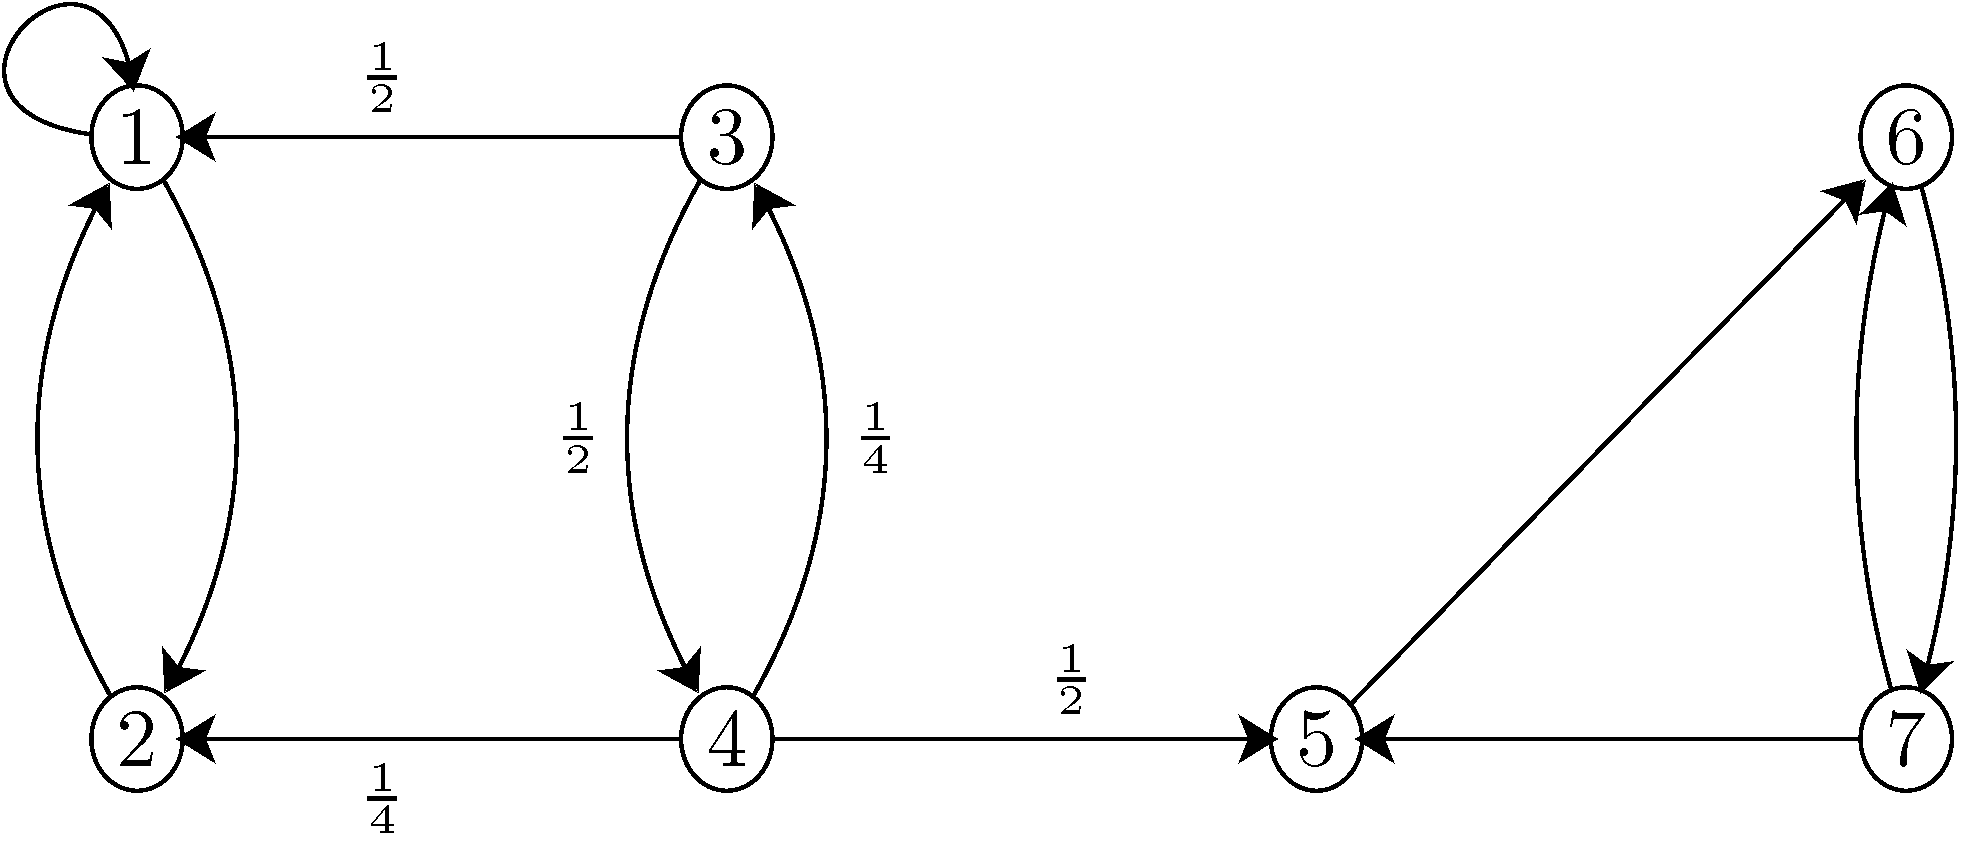
\includegraphics[width=10cm]{img/MC-diagram-rec-abs}
    % \caption{Рисунок к задаче \ref{mc_task1}.}
    % \label{fig:task}
    % \end{figure}

    \item Дана матрица перехода 
    \[
    P = \begin{pmatrix}
    \alpha & 1-\alpha\\
    \beta & 1 - \beta
    \end{pmatrix}.
    \]
    Найти $P^n$.

    % \item Игрок вступает в игру с капиталом $100\$$. В каждом ходу игры игрок получает $1\$$ с вероятностью $p$ и теряет $1\$$ с вероятностью $1-p$. Игра продолжается, пока игрок не наберёт $300\$$ или не проиграет все деньги. Какова вероятность, что игра когда-нибудь закончится? Какова вероятность, что игрок выйдет победителем?

    % \item \label{mc_task4} Рассмотрим марковскую цепь, показанную
    % на рисунке \ref{fig:task2}. Положим $\frac{1}{2} < p < 1$.
    % Есть ли у данной цепи предельное распределение? Найти
 %    \[
 %    \lim\limits_{n \to \infty} \Proba (X_n = j | X_0 = i).
 %    \]
    
 %    \begin{figure}[h!]
    %   \centering
    %   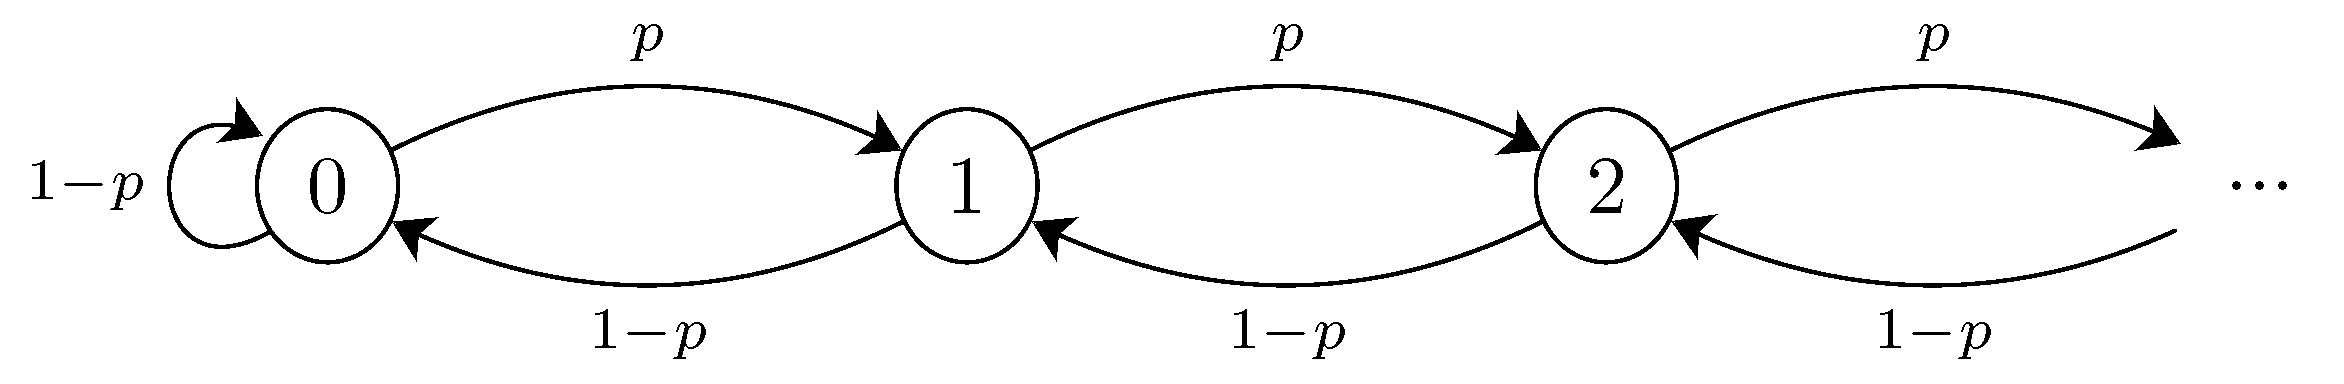
\includegraphics[width=10cm]{img/MC-diagram-inf-2}
    %   \caption{Рисунок к задаче \ref{mc_task4}.}
    %   \label{fig:task2}
    % \end{figure}

    \item Доказать, что функция $R(t, s) = \min\{t, s\} - ts$
     может или не может являться ковариационной функцией случайного процесса.

    \item Доказать, что функция $R(t, s) = \min\{t, s\} - t(s + 1)$
     может или не может являться ковариационной функцией случайного процесса.

    % \item Пусть $\newprocess{B}$ -- винеровский процесс. Доказать,
    % что процесс
    % \[
    % C_t = 
    %   \begin{cases}
    %       0, \quad & t = 0, \\
    %       t B_{1/t}, \quad & t > 0.
    %   \end{cases}
    % \]
    % также винеровский.

    % \item Пусть $\newprocess{B}$ -- винеровский процесс. Доказать,
    % что процесс
    % \[
    % C_t = 
    %   \sqrt{c} B_{t/c}, \qquad c = \mathrm{const} > 0
    % \]
    % также винеровский.

    % \item $\xi_1, \ldots, \xi_n$ -- независимые одинаково распределенные 
    % показательные случайные величины.
    % Подсчитать (по индукции) плотность распределения суммы
    % $\xi_1 + \ldots + \xi_n$.

    \item Пусть $\newprocess{N}$ -- пуассоновский случайный
    процесс с параметром $\lambda$. Доказать, что случайный
    процесс $\newprocess{M}$, задаваемый соотношением
    $M_t = N_{t+1} - N_t$, является стационарным второго порядка
    процессом, т.е. что его математическое ожидание $\Expect M_t$
    не зависит от времени, а его ковариационная функция
    $R_M(t_1, t_2)$ зависит от $t_1$ и $t_2$ через их разность
    $\tau = t_1 - t_2$.

    % \item Доказать положительную определенность функции
    % \[
    % R(t, s) = 
    %       \begin{cases}
    %           1 - |t - s|, \quad & |t - s| < 1, \\
    %           0, \quad & |t - s| >= 1.
    %       \end{cases}
    % \]

    % \item Доказать положительную определенность функции
    % \[
    % R(t, s) = e^{- |t - s|}.
    % \]

    % \item Пусть $\xi_1, \xi_2, \ldots$ -- независимые одинаково
    % распределенные случайные величины, причем
    % $\Proba (\xi_t = 1) = p, \Proba (\xi_t = -1) = 1 - p$.
    % Является ли цепью Маркова последовательность
    % $\eta_t = \xi_t \xi_{t + 1}$? Если да, 
    % найти ее вероятности перехода за один шаг.

    \item Пусть $\xi_1, \xi_2, \ldots$ -- независимые одинаково
    распределенные случайные величины, причем
    $\Proba (\xi_t = 1) = p, \Proba (\xi_t = -1) = 1 - p$.
    Является ли цепью Маркова последовательность
    $\eta_t = \xi_1 \xi_2 \ldots \xi_t$? Если да, 
    найти ее вероятности перехода за один шаг.

    % \item Для случайного процесса $\newprocess{h}$, заданного выражением
    % \[
    % h_t = \varepsilon_t - 1.3 \varepsilon_{t-1} + 0.4 \varepsilon_{t-2},
    % \]
    % где $\newprocess{\varepsilon}$ -- последовательность независимых
    % одинаково стандартно нормально распределенных случайных величин,
    % \begin{enumerate}
    % \item Провести исследование на стационарность 2-го порядка (с доказательством);
    % \item Вычислить первые четыре автокорреляции $\rho_0, \rho_1, \rho_2, \rho_3$;
    % \item Вычислить дисперсию случайной величины $h_t$.
    % \end{enumerate}

    % \item Для случайного процесса $\newprocess{h}$, заданного выражением
    % \[
    % h_t - h_{t-1} = \varepsilon_t - 1.3 \varepsilon_{t-1} + 0.3 \varepsilon_{t-2},
    % \]
    % где $\newprocess{\varepsilon}$ -- последовательность независимых
    % одинаково стандартно нормально распределенных случайных величин,
    % \begin{enumerate}
    % \item Провести исследование на стационарность 2-го порядка (с доказательством);
    % \item Вычислить первые четыре автокорреляции $\rho_0, \rho_1, \rho_2, \rho_3$;
    % \item Вычислить дисперсию случайной величины $h_t$.
    % \end{enumerate}

    \item Для модели GARCH(1, 1) временного ряда, задающейся уравнениями
    \begin{align*}
    X_n = \mu + h_n, 
    \quad 
    h_n = \sigma_n \varepsilon_n, \\
    \sigma_n^2 = \alpha_0 + \alpha_1 h_{n-1}^2 + \beta_1 \sigma_{n-1}^2,
    \end{align*}
    где $\newprocessd{\varepsilon}$ -- процесс гауссовского белого шума,

    \begin{enumerate}
    \item Записать формулу для подсчета $\sigma^2_{n+1}$;
    \item Подсчитать распределение величины $X_{n+1}$.
    \end{enumerate}

\end{enumerate}


\end{document}
